
\newcommand{\argmaxs}[2]{\arg \max_{#2}{#1}}

\section{Exercises}

\subsection{Bayes}
\begin{figure}[H]
    \centering
    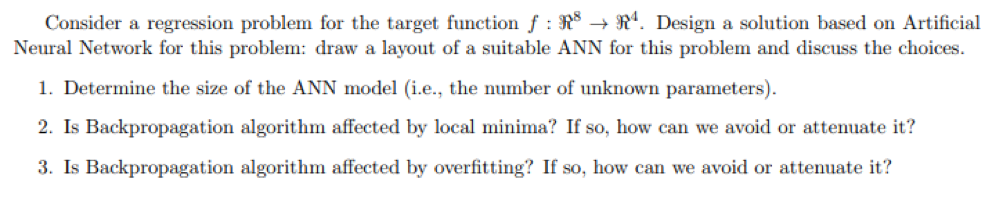
\includegraphics[scale=1]{exercises/ex1.png}
\end{figure}


In Multinomial Naïve Bayes each $p(c)$ is a multinomial distribution, so it is possible to solve the classification problem of documents using Multinomial Naïve Bayes because multinomial distribution works well for data which can easily be turned into counts, such as word counts in a text.
Given:
\begin{itemize}
\item $P(c_j)$: probability of class $c_j$
\item $P(w_i|c_j)$: probability of the word $w_i$ given the class $c_j$.
\end{itemize}
We must estimate $P(c_j)$ and $P(w_i|c_j)$ using multinomial distribution, then use them to classify a new document. Remove every word in the documents not appearing in the vocabulary V build in the previous phase and then use:
\[V_{NB}=\argmaxs{P(c_j)\prod_{i=1}^{lenght(d)}P(w_i|c_j,D)}{c_j \in C}\]

\subsection{Markov}
\begin{figure}[H]
    \centering
    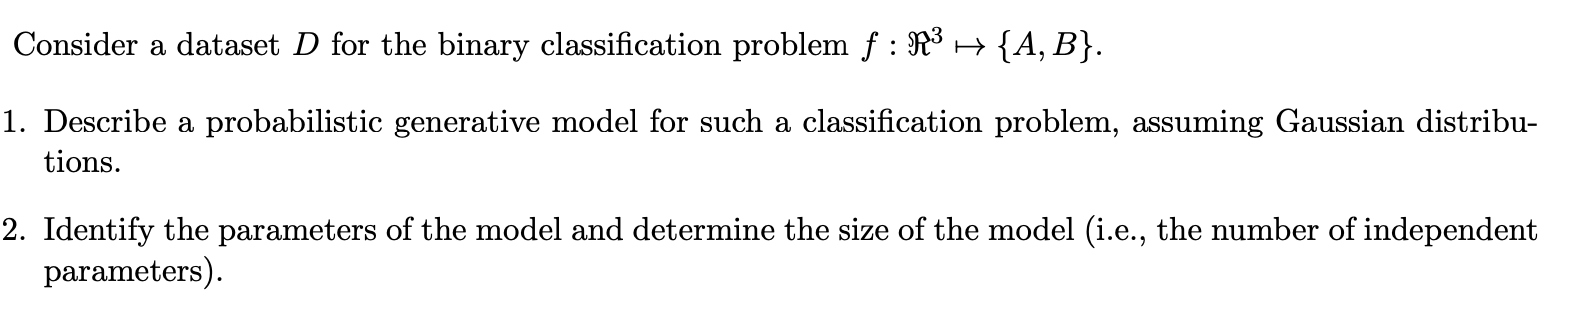
\includegraphics[scale=1]{exercises/ex2.png}
\end{figure}

\paragraph{Markov properties} once the current state is known, the evolution of the dynamic system does not depend on the history of states, actions and observations. The current state contains all the information needed to predict the future. Future states are conditionally independent of past states and past observations given the current state. The knowledge about the current state makes past, present and future observations statistically independent. Markov process has Markov properties.\\


\paragraph{MDP}
\begin{figure}[H]
    \centering
    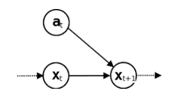
\includegraphics[scale=1]{MDP.png}
\end{figure}

An MDP is for decision making where the states are fully observable, hence there is  no need of observations. In presence of non-deterministic or stochastic actions, they can be fully observed after its execution.\\
Having 
\begin{itemize}
\item $X$ finite set of states:
\item $A$: finite set of actions
\item Deterministic $\delta: X\times A \rightarrow X$: a function which maps an action-state tuple to the next state.
\item Non-deterministic $\delta: X\times A \rightarrow 2^X$.
\item Stochastic $\delta: P(x'|x,a)$: the probability of having he state $x'$ given previous state $x$ and action $a$.
\item Deterministic $r:X\times A \rightarrow R$: a function which maps a tuple state-action to a reward.
\item Non-deterministic/Stochastic $r:X\times A \times X \rightarrow R$
\end{itemize}
An MDP is made of $MSP=\braces{X,A,\delta,r}$

\paragraph{HMM}
\begin{figure}[H]
    \centering
    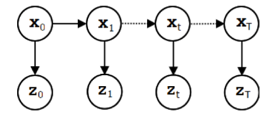
\includegraphics[scale=1]{HMM.png}
\end{figure}

In a HMM sate states $x_t$ are discrete and not observable, while the observations $z_t$ can be either discrete or continuous. Finally there is no control over the system.\\
Given:
\begin{itemize}
\item $X$: set of not observable states
\item $Z$: set of observations
\item $P(x_t|x_{t-1})$: the transition model 
\item $P(z_t|x_t)$: an observation models which maps the probability of having an observation $z_t$ to a state $x_t$.
\item $\pi_0$: an initial distribution
\item $\bm{A}=\braces{A_{ij}}=P(x_t=j|x_{t-1}=i)$ a transition matrix
\item $b_k(z_t)=P(z_t|x_t=k)$ an observation model.
\item $\pi_0=P(x_0)$: an initial probability.
\end{itemize}
We have that a HMM is made of $HMM=\braces{X,Z,\pi_0}$.

\subsection{Kernelized linear model (regression)}
\begin{figure}[H]
    \centering
    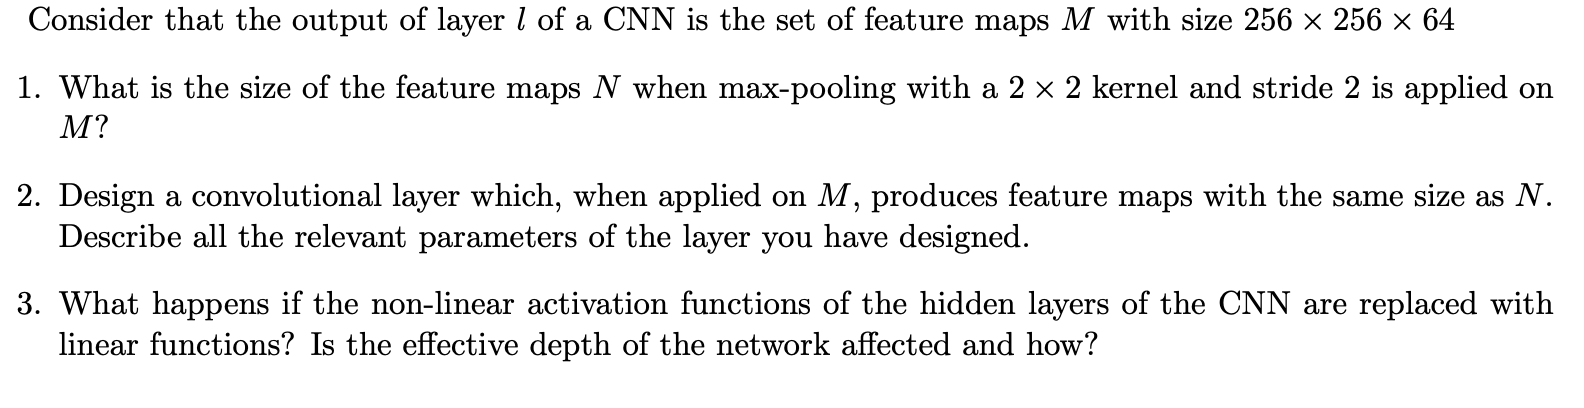
\includegraphics[scale=1]{exercises/ex3.png}
\end{figure}

\paragraph{Gram Matrix}
Given some kernel $k(x_i,x_j)$, the Gram Matrix $K=\bm{XX^T}$ is a $N\times N$ symmetric matrix of the form:
\[K_{nm}=k(x_n,x_m)\]

\paragraph{Kernalized regression}
Considering a linear kernel $k(x,x')=x^Tx'$ we can rewrite the model as:
\[y(x)=\sum_{i=1}^N\alpha_i k(x_i,x)\]
having:
\[\alpha=(K+\lambda I)^{-1}t\]

\subsection{Linear Regression}

\begin{figure}[H]
    \centering
    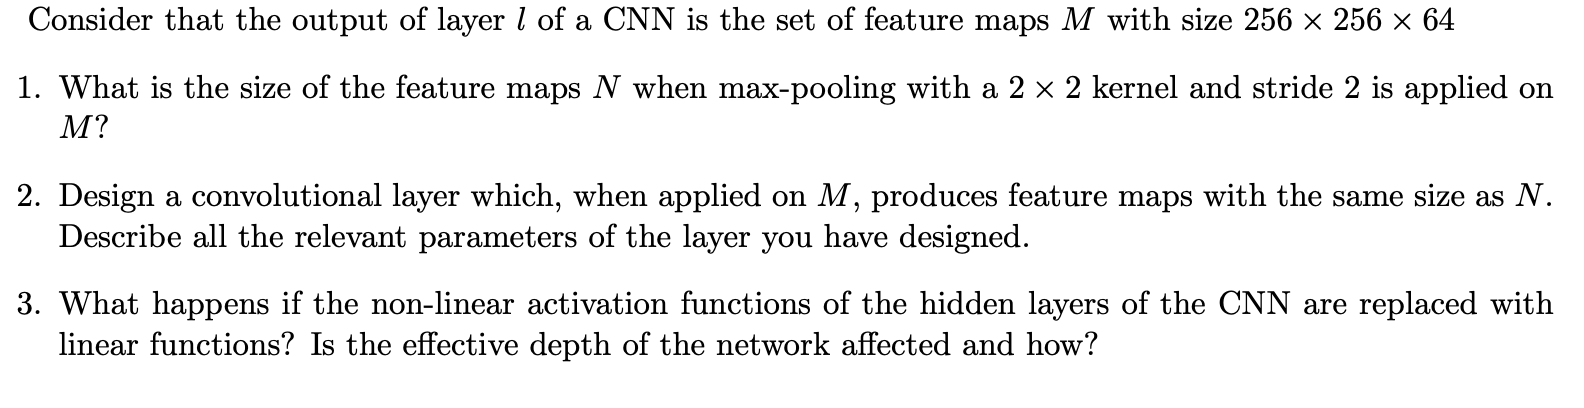
\includegraphics[scale=1]{exercises/ex3.png}
\end{figure}


\paragraph{Linear regression}
The goal of regression is to predict the value of one or more continuous target variables $Y=\mathcal{R}$ given the value of a D-dimensional vector of input variables $X \subset \mathcal{R}^D$. The simplest linear model for regression is one that involves a linear combination of the input variables:
\[y(x,w)=w_0+w_1x_1+...+w_Dx_D=\bm{w^Tx}\]
Where $x_0=1$.

\paragraph{Batch vs sequential}


We have that a target value is given by:
\[t=y(x,w) + \epsilon\]
Where $\epsilon$ is some Gaussian noise. If we assume the samples to be i.i.d. then we can use the maximum likelihood and have:
\[max[P(\braces{t_1,...,t_n}|x_1,...,x_n,w,\beta)]\]
where $\beta^{-1}$ is the variance of the noise. This approach is used with batch learning in which the entire training set is processed altogether.\\

For sequential learning \textit{stochastic gradient descent} can be used to update the model parameters in the following way:
\[w_{n+1}=w_n+\eta \nabla E_n= w_n +[t_n -w_n^T \phi(x_n)]\phi(x_n)\]
Where:
\begin{itemize}
\item $\eta$: is the learning rate 
\item $\phi(x_n)$ : is a non linear transformation of the input vector
\end{itemize}



\subsection{Linear classification}

\begin{figure}[H]
    \centering
    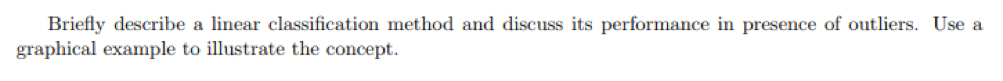
\includegraphics[scale=1]{exercises/ex5.png}
\end{figure}

The goal in classification is to take an input vector $x$ and to assign it to one of $K$  discrete classes $C_k$ where $k=1,...,K$. In the most common scenario, the classes are taken to be disjoint, so that each input is assigned to one and only one class. Data sets whose classes can be separated exactly by linear decision surfaces are said to be linearly separable. There are various ways of using target values to represent class labels.\\
For probabilistic models, the most convenient, in the case of two-class problems, is the binary representation in which there is a single target variable $t \in \braces{0,1}$ such that $t=1$ represents class $C_1$  and $t=0$  represents class $C_2$. The value of $t$ can be viewed as representing the probability of belonging to the class $C_1$.\\
For $K>2$  it is convenient to use a 1-of-K coding scheme, which is a vector $T=\braces{t_1,t_2,...,t_n}$ of length $K$ such that if the class is $C_j$, for some sample $x_i \in X,\ |X|=n$ , then the value of $t_i$ is zero everywhere except for $t_i^j$ which is one. \\
Given a dataset in the form $D=\braces{(x_n,t_n)^N_{n=1}}$ we want to find a linear discriminant $y(x)=W^Tx$, hence we minimize the sum of squares error function:
\[E(W)=\frac{1}{2}Tr\braces{(XW-T)^T(XW-T)}\]
obtaining:
\[W=(X^TX)^{-1}X^TT\]
\[y(x)=W^Tx\]
Unfortunately, least squares solutions lack robustness to outliers and are highly sensitive to them, unlike logistic regression.

\begin{figure}[H]
    \centering
    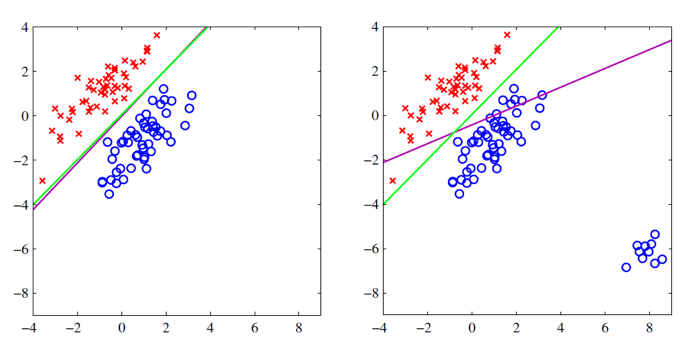
\includegraphics[scale=1]{least_square_error.png}
\end{figure}
The left plot shows data from two classes (red crosses and blue circles) with the decision boundary found by least squares (magenta) and by the logistic regression model (green). The right plot shows the corresponding results obtained when extra data points (outliers) are added at the bottom left of the diagram.

\subsection{K-NN}

\begin{figure}[H]
    \centering
    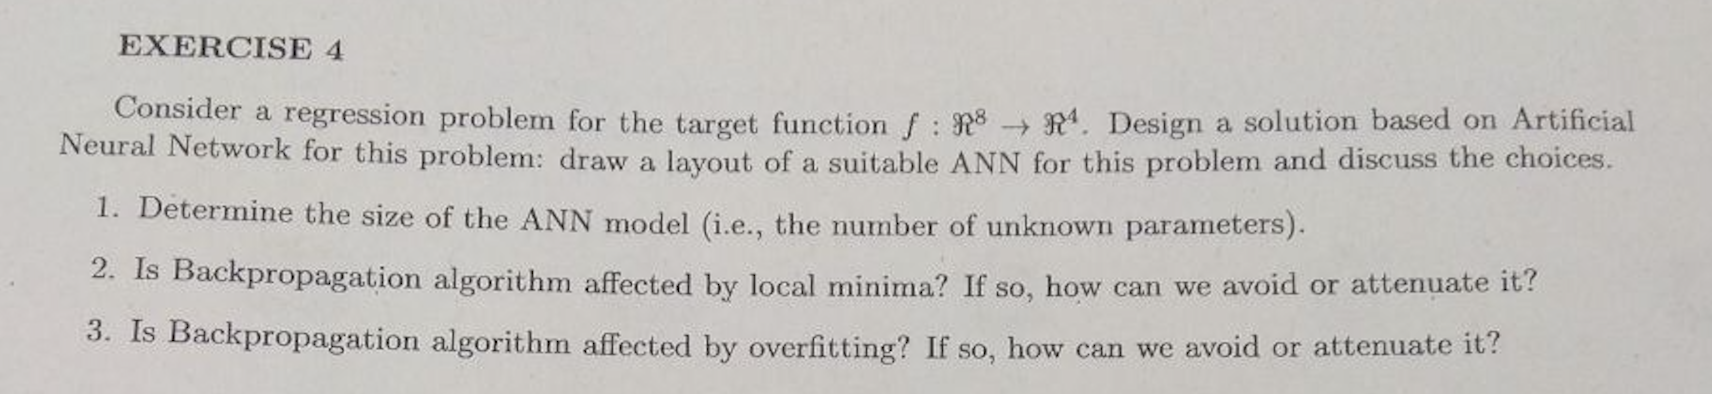
\includegraphics[scale=1]{exercises/ex6.png}
\end{figure}

\paragraph{Main steps}
Classification with K-NN, having a target function $f:X\rightarrow C$ and a dataset $D=\braces{(x_i,y_i)^N_{i=1}}$ is :
\begin{itemize}
\item Find K nearest neighbors of the new instance $x'$
\item assign $x'$ to the most common label among the majority of the neighbors.
\end{itemize}
We can estimate the likelihood of $x'$ belongign to the class $c$ as:
\[p(c| x',D,K)=\frac{1}{K}\sum_{i \in N_k(x',D)}\mathcal{I}(y_i=c)\]
with:
\begin{itemize}
\item $ N_k(x',D)$ is the set of K nearest points to $x'$
\item $\mathcal{I}(y_i=c)$ is one if the label $y_i$ is equal to $c$, zero otherwise
\end{itemize}

\paragraph{Exercise}
\begin{figure}[H]
    \centering
    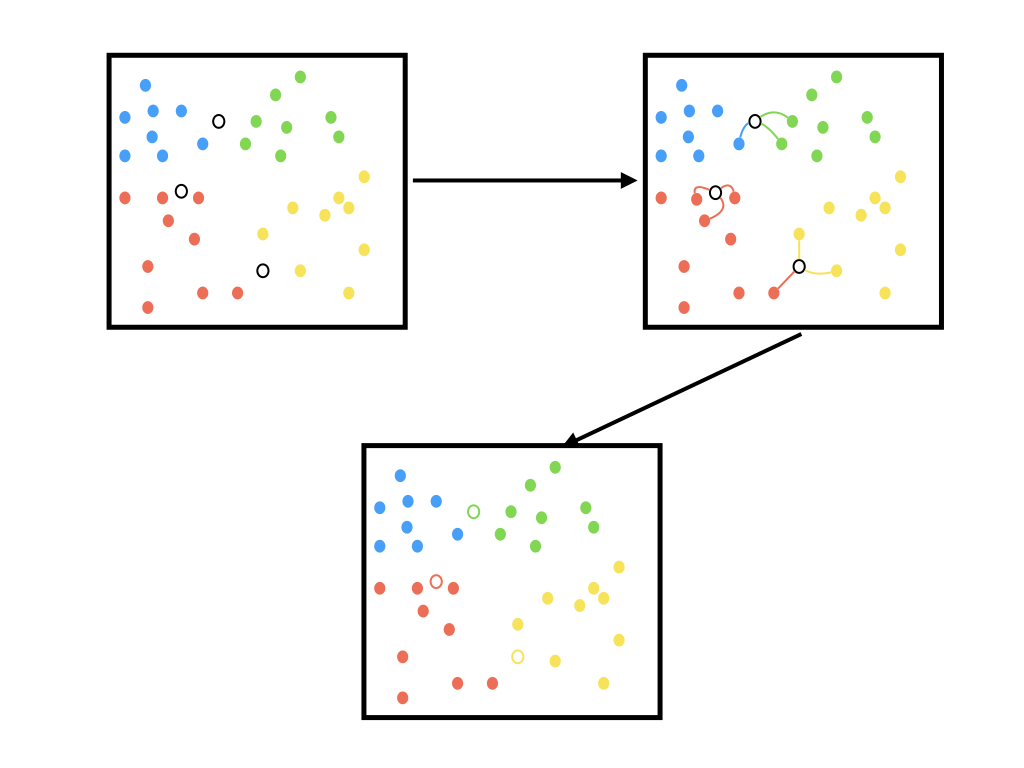
\includegraphics[scale=0.4]{knn.jpeg}
\end{figure}
\subsection{Tree classification}
\begin{figure}[H]
    \centering
    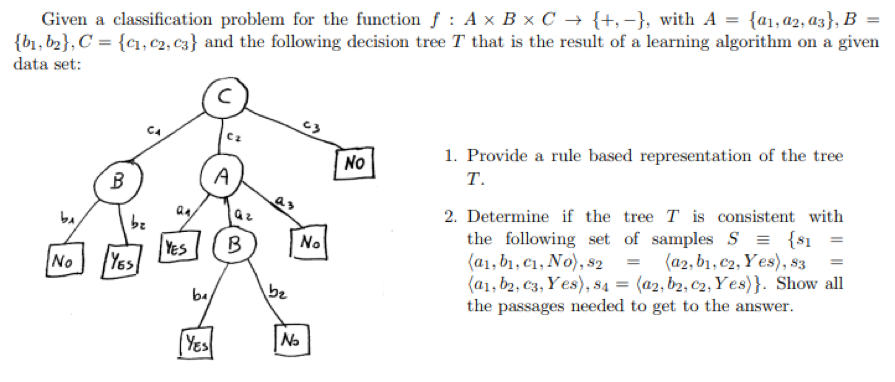
\includegraphics[scale=1]{exercises/ex7.png}
\end{figure}

\paragraph{Rules}
\begin{enumerate}

\item $c_1 \wedge b_1 \Rightarrow No $
\item $c_1 \wedge b_2 \Rightarrow Yes $
\item $c_2 \wedge a_1 \Rightarrow Yes $
\item $c_2 \wedge a_2 \wedge b_1 \Rightarrow Yes $
\item $c_2 \wedge a_2 \wedge b_2 \Rightarrow No $
\item $c_2 \wedge a_3 \Rightarrow No $
\item $c_3  \Rightarrow No $
\end{enumerate}

\paragraph{Consistency}
\begin{itemize}
\item $s_1$ is consistent because of  1 
\item $s_2$ is consistent because of  4
\item $s_3$ is not consistent because of  7 
\item $s_4$ is not consistent because of  5
\end{itemize}

\subsection{Tree overfitting}
\begin{figure}[H]
    \centering
    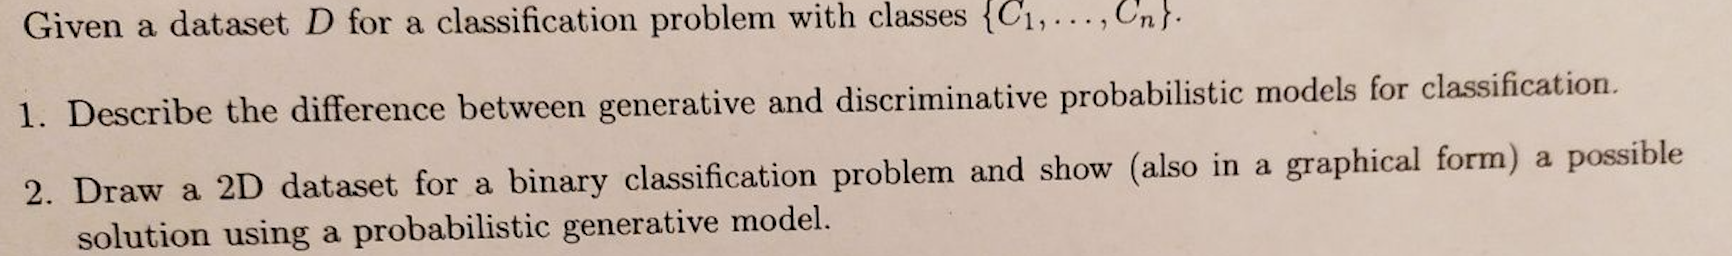
\includegraphics[scale=1]{exercises/ex8.png}
\end{figure}


\paragraph{Overfitting}
Overfitting is "the production of an analysis that corresponds too closely or exactly to a particular set of data, and may therefore fail to fit additional data or predict future observations reliably". An overfitted model is a statistical model that contains more parameters than can be justified by the data.[2] The essence of overfitting is to have unknowingly extracted some of the residual variation (i.e. the noise) as if that variation represented underlying model structure.

\paragraph{Overfitting in Tree}
Consider an hypothesis $h$ with error on the training set $error_{train}(h)$, while the error on the enitre distribution D is $error_D(h)$. The hypo $h$ overfits the training data if there is some other hypo $h'$ and the following holds:
\[error_{train}(h)<error_{train}(h')\quad and \quad error_D(h)>error_D(h')\]
stop growing when data split is not statistically significant, acquire more training data, remove irrelevant attributes, grow full tree, then post-prune. In order to select the best tree, we have to measure performance over training data, measure performance over separate validation data set, add complexity penalty to performance measure.

\subsection{Boosting}
\begin{figure}[H]
    \centering
    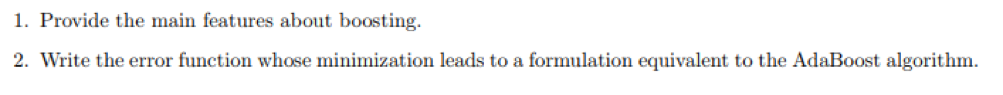
\includegraphics[scale=1]{exercises/ex9.png}
\end{figure}

\paragraph{Boosting}
In supervised learning, boosting converts weak learners to strong ones. A weak learner is defined to be a classifier that is only slightly correlated with the true classification (it can label examples better than random guessing). In contrast, a strong learner is a classifier that is arbitrarily well-correlated with the true classification.

\paragraph{AdaBoost}
No prior knowledge about base learner is required, no parameters to tune (except for M), can be combined with any method to find base learners and theoretical guarantees given enough data and base learners with moderate accuracy.\\
The error function to minimize is:
\[J_m=\sum_{n=1}^N w_n^{(m)}\mathcal{I}(y_m(x_n)\neq t_n\]
Given 
\begin{itemize}
\item $\epsilon_m = \frac{\sum_{n=1}^N w_n^{(m)}\mathcal{I}(y_m(x_n)\neq t_n}{\sum_{n=1}^N w_n^{(m)}}$
\item $\alpha=ln(\frac{1-\epsilon_m}{\epsilon_m})$
\end{itemize}
The output of the linear classifier is:
\[Y_m(x)=sign(\sum_{m=1}^M\alpha_my_m(x))\]


\begin{figure}[H]
    \centering
    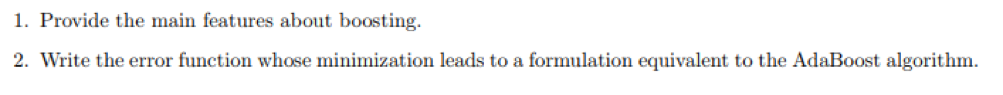
\includegraphics[scale=1]{exercises/ex9.png}
\end{figure}

\paragraph{Boosting}
In supervised learning, boosting converts weak learners to strong ones. A weak learner is defined to be a classifier that is only slightly correlated with the true classification (it can label examples better than random guessing). In contrast, a strong learner is a classifier that is arbitrarily well-correlated with the true classification.

\paragraph{AdaBoost}
No prior knowledge about base learner is required, no parameters to tune (except for M), can be combined with any method to find base learners and theoretical guarantees given enough data and base learners with moderate accuracy.\\
The error function to minimize is:
\[J_m=\sum_{n=1}^N w_n^{(m)}\mathcal{I}(y_m(x_n)\neq t_n\]
Given 
\begin{itemize}
\item $\epsilon_m = \frac{\sum_{n=1}^N w_n^{(m)}\mathcal{I}(y_m(x_n)\neq t_n}{\sum_{n=1}^N w_n^{(m)}}$
\item $\alpha=ln(\frac{1-\epsilon_m}{\epsilon_m})$
\end{itemize}
The output of the linear classifier is:
\[Y_m(x)=sign(\sum_{m=1}^M\alpha_my_m(x))\]

\subsection{Unsupervised vs supervised}
\begin{figure}[H]
    \centering
    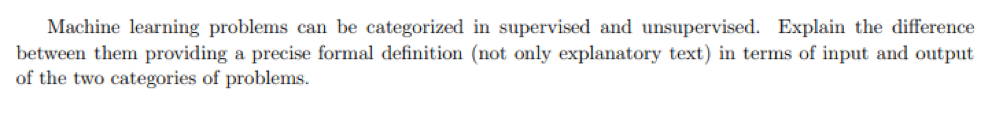
\includegraphics[scale=1]{exercises/ex10.png}
\end{figure}

Supervised learning is typically done in the context of:
\begin{itemize}
\item \textbf{Classification}: when we want to map input to output labels.
\item \textbf{Regression}: when we want to map input to a continuous output.
\end{itemize} 

In both regression and classification, the goal is to find specific relationships or structure in the input data that allow us to effectively produce correct output data.\\

Unsupervised learning uses techniques such as clustering, representation learning and density estimation. In all of these cases, we wish to learn the inherent structure of our input data without using explicitly-provided labels. Since no labels are provided, when analyzing the output there is no specific way to compare model performance in most unsupervised learning methods.\\
 
On the other hand, supervised learning  intends to infer a conditional probability distribution $p_X(x|y)$ conditioned on the label $y$ of input data; unsupervised learning intends to infer an a priori probability distribution $P_X(x)$ . Compared to supervised learning where training data is labeled with the appropriate classifications, models using unsupervised learning must learn relationships between elements in a data set and classify the raw data without "help."

\subsection{Unsupervised}
\begin{figure}[H]
    \centering
    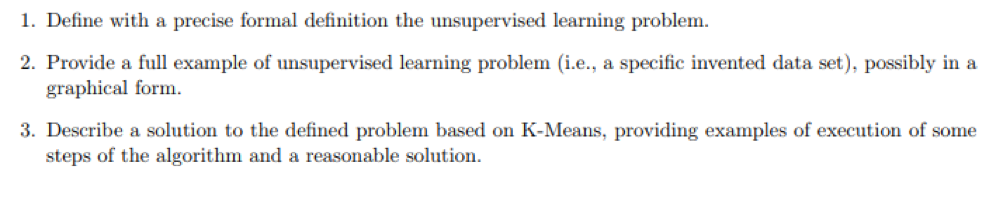
\includegraphics[scale=1]{exercises/ex11.png}
\end{figure}

\paragraph{Definition}
Unsupervised learning is a branch of machine learning that learns from test data that has not been labeled, classified or categorized. Instead of responding to feedback, unsupervised learning identifies commonalities in the data and reacts based on the presence or absence of such commonalities in each new piece of data. Alternatives include supervised learning and reinforcement learning. 

\paragraph{Example}
Using K-Means with number of clusters equal to 4, we get 

\begin{figure}[H]
    \centering
    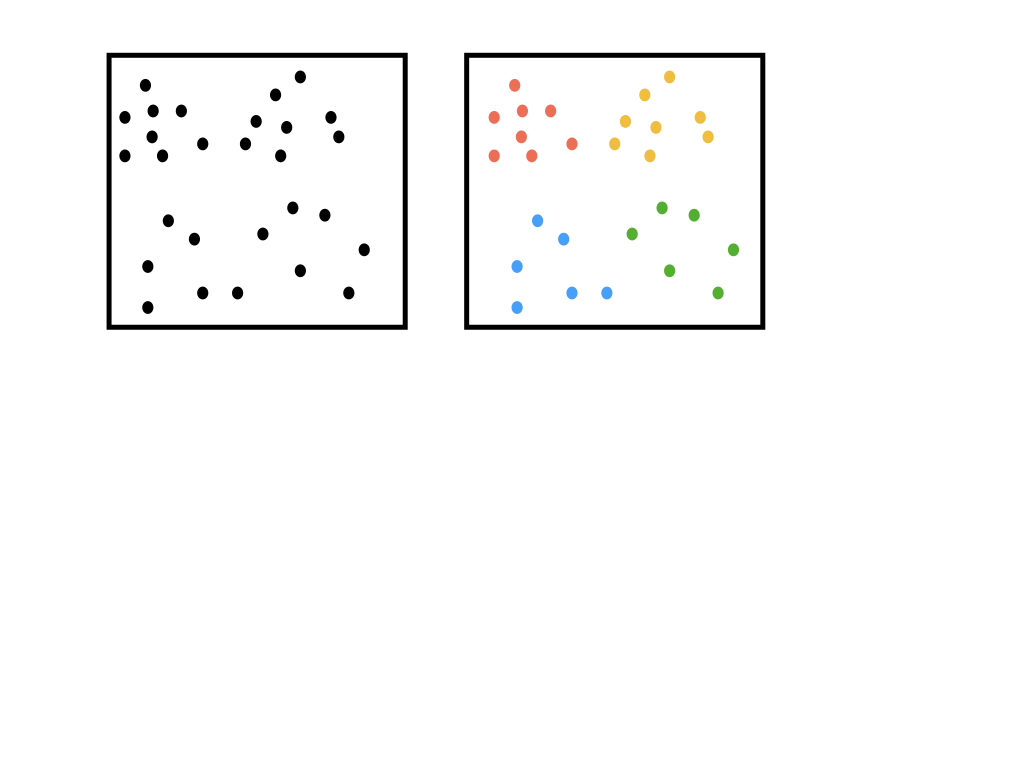
\includegraphics[scale=0.4]{kmeans.jpeg}
\end{figure}

\paragraph{K-Means}
Nope
\subsection{ANN}
\begin{figure}[H]
    \centering
    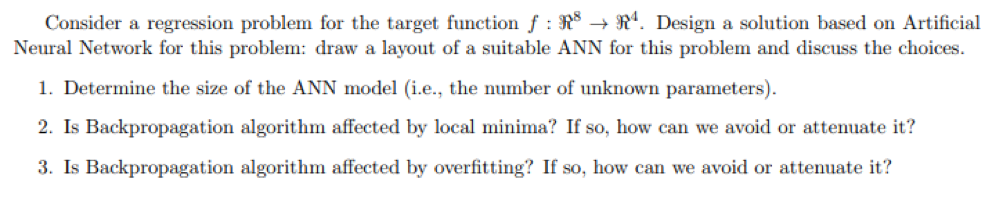
\includegraphics[scale=1]{exercises/ex12.png}
\end{figure}

\subsection{ANN2}
\begin{figure}[H]
    \centering
    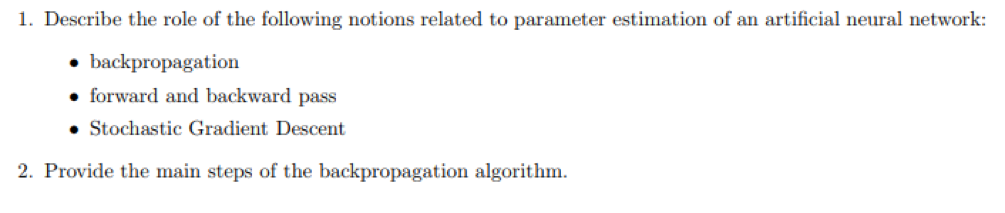
\includegraphics[scale=1]{exercises/ex13.png}
\end{figure}

\paragraph{Back-Propagation}
Backpropagation algorithm is used to propagate gradient computation from the cost through the whole network. The goal is to compute the gradient of the cost function w.r.t. the parameters $\nabla_{\theta}J(\theta)$ in a simple and efficient way.

\paragraph{Backward and Forward pass}
The forward pass computes values from inputs to output and the backward pass then performs backpropagation which starts at the end and recursively applies the chain rule to compute the gradients all the way to the inputs of the circuit. The gradients can be thought of as flowing backwards through the circuit.


\paragraph{Stochastic Gradient Descend}
Stochastic Gradient Descent updates the weight parameters after evaluation of the cost function after each sample.  That is, rather than summing up the cost function results for all the sample then taking the mean, SGD updates the weights after every training sample is analysed.

\paragraph{Back-Propagation algorithm}
